%%%%%%%%%%%%%%%%%%%%%%%%%%%%%%%%%%%%%%%%%%%%%%%%%%%%%%%%%%%%
%% Chapter 2 — Fundamentals and Related Work (12–18 pages)
%% Purpose: provide only the theory and literature needed to
%% understand the research choices, then end with the
%% unresolved gap addressed by the thesis.
%%%%%%%%%%%%%%%%%%%%%%%%%%%%%%%%%%%%%%%%%%%%%%%%%%%%%%%%%%%%
\chapter{Fundamentals and Related Work}
\label{chap:fundamentals}

Chapter~\ref{chap:introduction} argued that precise task-space tracking
with a hydraulic mowing arm is limited less by kinematics than by the
actuator. The path from a valve command to actual cylinder motion is
nonlinear and load dependent, and it differs from one machine, season, or
attachment to the next. This chapter collects the background needed to
judge that argument and to understand the design decisions made later in
the thesis. Section~\ref{sec:fund:actuation} introduces the machine class
and its electro-hydraulic actuation. Section~\ref{sec:fund:kinematics}
recalls the kinematic tools behind the classical controller, and
Section~\ref{sec:fund:conventional-control} reviews how conventional
model-based control deals with hydraulic uncertainty. The remaining sections cover the learning methods this work builds on.
Section~\ref{sec:fund:learned-dynamics} treats data-driven dynamics models and
the pitfalls of identifying them from closed-loop data.
Section~\ref{sec:fund:rom} covers reduced-order and grey-box modeling,
Section~\ref{sec:fund:domain-randomization} domain randomization and latent
adaptation, and Section~\ref{sec:fund:rl-residual} policy optimization with
structured priors.
Section~\ref{sec:fund:gap} then states the gap that remains and how the
three control stacks of this thesis (\ppoROM, \ppoIDFD, and
\ppoIDAAMFD) address it. Only material that is
needed for the later chapters is included. The concrete system definition
and problem formulation follow in Chapter~\ref{chap:system}.

\section{Manipulator Actuation and Control Fundamentals}
\label{sec:fund:actuation}

\subsection{Application Context and Implement Carriers}

The machine studied in this thesis belongs to a class that is easy to
overlook because it is so common: hydraulic booms mounted on road-going
implement carriers, doing repetitive maintenance work along traffic
infrastructure. Section~\ref{sec:sys:platform} shows the concrete instance,
the MULAG FME~500 front mower on a Unimog
carrier~\cite{mulag2024fme500}. A multi-link boom carries a
$\unit[1.2]{m}$ flail mowing head to the roadside verge, reaches up to
about $\unit[6.5]{m}$ to either side of the vehicle, and must hold the
head in a shallow band above the ground while the vehicle creeps along
the road. The manufacturer's working envelope, reproduced in
Figure~\ref{fig:sys:fme500}, makes the difficulty concrete. The same arm that mows a flat verge beside the
wheels must also reach over guardrails, down embankments to about
$\unit[3]{m}$ below road level, and up to $\unit[8]{m}$ for hedge work,
with the same linkage and the same operator. In practice, head height,
tilt, and lateral position are adjusted continuously by a human through
open-loop joystick commands. It is skilled and fatiguing work, done while
also driving the vehicle. Automating the tracking part of this task is
the practical motivation of this thesis.

Hydraulic actuation dominates this machine class for reasons that remain
valid despite the rise of electric drives. Cylinders deliver very high
force from small, rugged, and inexpensive components; they tolerate shock
loads such as the mowing head striking a curbstone; and the carrier
vehicle already provides hydraulic power through its power take-off. The
price is paid in controllability. An electric joint drive responds to
current within milliseconds and nearly linearly. A hydraulic cylinder
responds through a chain of nonlinear energy conversions whose effective
gain can change by an order of magnitude across the workspace. Mattila et
al.~\cite{mattila2017survey} survey two decades of research on this
tension between the force density of hydraulic manipulators and the
difficulty of controlling them precisely.

\subsection{The Electro-Hydraulic Actuation Chain}
\label{sec:fund:actuation-chain}

\begin{figure}[tb]
  \centering
  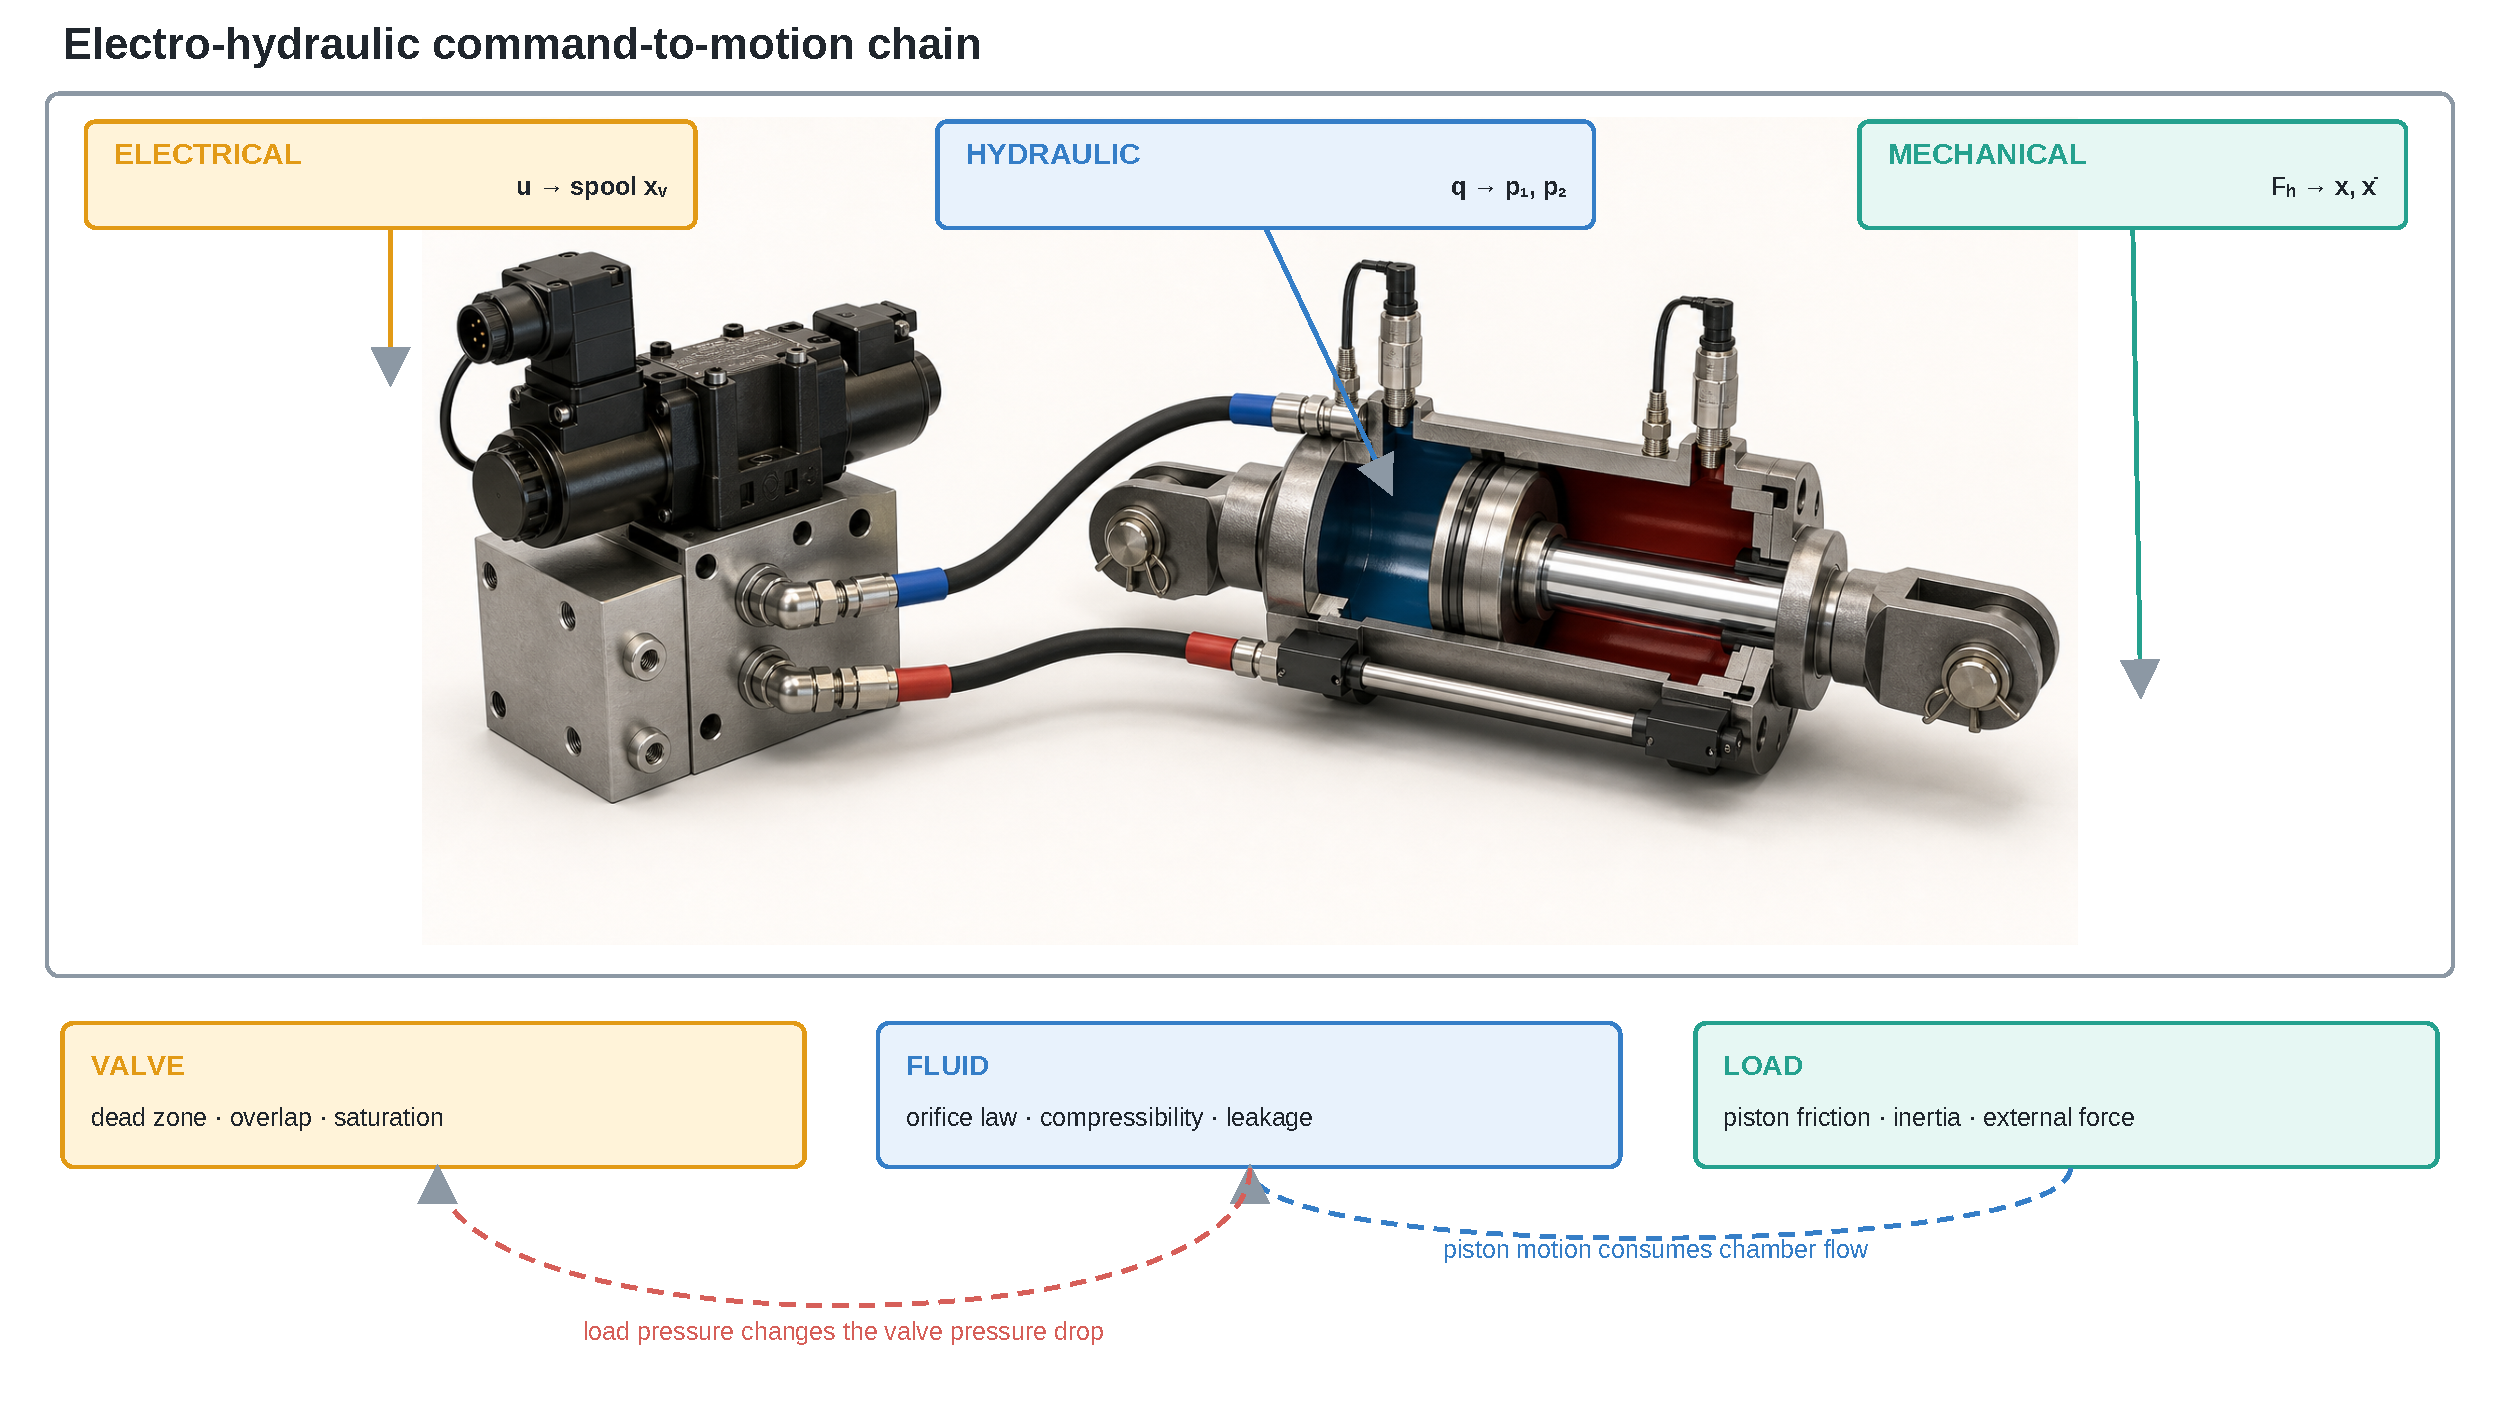
\includegraphics[width=\textwidth]{images/fund_actuation_chain}
  \caption{The electro-hydraulic actuation chain from valve command to
  mowing-head motion, grouped by energy domain. Tags beneath each domain name
  its dominant nonlinearities. The dashed return paths are the feedback loops
  that make the chain gain an operating point rather than a constant.}
  \label{fig:fund:chain}
\end{figure}

Figure~\ref{fig:fund:chain} traces the signal path that every command to
the arm must traverse. A normalized electrical command displaces the
spool of a proportional valve, which opens metering orifices toward the
supply and tank lines. To first approximation the resulting flow follows the orifice
law~\cite{merritt1967hydraulic}, in which the flow through the valve is
proportional to the spool position and to the square root of the pressure
difference across the metering edge, scaled by the discharge coefficient and
the orifice area gradient. The form is written out in
Section~\ref{sec:sys:simscape} with the coefficient values used by the plant
model. Two of its properties shape everything that follows in this thesis.
First, the flow gain depends on the square root of the pressure margin. The same spool
displacement therefore moves the cylinder quickly under light load and
barely at all when the load pressure approaches supply. The effective
valve authority is an operating point, not a constant. Second, the
relation is directional. Extending against gravity and retracting with it
see different pressure margins and hence different gains. Around the
spool null, machining overlap produces a dead zone in which small
commands move nothing at all, and at the other end of the stroke the
spool saturates~\cite{jelali2003hydraulic}.

The delivered flow does not translate directly into motion either. Oil
is compressible, the more so when air is entrained, so each cylinder
chamber acts as a nonlinear spring. Its stiffness scales with the
effective bulk modulus and inversely with the chamber volume, and the
volume itself changes with piston position. Pressure relief valves clip
the dynamics whenever a load spike or an aggressive command drives a
chamber to its limit, which happens routinely in mowing when the head
rests on the ground. Internal leakage bleeds pressure between chambers,
seal friction opposes motion, and the load pressure feeds back into the
valve flow through the orifice law. Taken together, this is the
plant that the learned models of this thesis must represent: several
interacting nonlinearities, some of them non-smooth (relief, dead zone,
stiction), and parameters such as bulk modulus, leakage, and friction
that drift with temperature and wear.

One structural point matters for the control architecture. The chain in
Figure~\ref{fig:fund:chain} ends in the mechanical linkage, where
cylinder translation becomes joint rotation through lever arms that vary
with configuration. Uncertainty entering at the valve is therefore
filtered, amplified, and coupled by the mechanism before it appears as
head-position error. This is why the models of Chapter~\ref{chap:models}
are formulated in \emph{cylinder space}, directly across the hydraulic
conversion stages, rather than in task space where hydraulic and
kinematic effects blur together.

\subsection{High-Fidelity Simulation as a Data Source}
\label{sec:fund:sim-data-source}

The hydraulic subsystems above can be modeled in detail in
component-level simulation environments such as
Simscape~\cite{mathworks2024simscape}, and Chapter~\ref{chap:data} builds
on such a model of the FME~500 arm. It is tempting to close the loop and
train a reinforcement-learning policy directly against this model, but
the computational profiles do not match. The stiff pressure dynamics
force small integration steps, and the solver processes one machine
instance at a time, while modern policy optimization spreads its sample
cost over thousands of plants simulated in parallel on a
GPU~\cite{makoviychuk2021isaac}. This thesis resolves
the mismatch by separation: the high-fidelity model is used offline as a
data generator, and compact learned representations of the actuator
carry its behavior into the parallel training environment. How this
workflow fits together is shown later, in
Figure~\ref{fig:fund:workflow}, once its ingredients have been
introduced.

\section{Kinematics and Task-Space Tracking}
\label{sec:fund:kinematics}

\subsection{Differential Kinematics}

The mowing task is specified where the work happens, as a reference path
for the cutter in vehicle coordinates. Task-space control therefore rests
on the differential kinematics of the arm~\cite{siciliano2009robotics},
in which the manipulator Jacobian maps joint rates to tool velocity and
its inverse yields the commands realizing a desired tool motion. The
plain pseudo-inverse is fragile near singular configurations, which this
arm visits routinely with the boom almost fully folded. The standard
remedy, adopted unchanged here, is the damped least-squares inverse of
Wampler~\cite{wampler1986manipulator} and Nakamura and
Hanafusa~\cite{nakamura1986inverse}, which trades bounded tracking
accuracy for bounded joint commands. It is conservative, well understood
and cheap, which are the properties wanted in a layer that must never
misbehave.

\subsection{From Joint Space to Cylinder Space}

Two complications specific to a hydraulic boom carry into the rest of the
thesis. The actuated coordinates are cylinder lengths rather than joint
angles, and each cylinder closes a triangle over its joint, so the
cylinder-to-joint map is nonlinear and its lever arm varies over the
stroke. The Jacobian used for control is therefore the composition of the
task Jacobian with that map, and an error in one cylinder's realized
motion appears in the task error of the whole arm. A passive fifth joint
coupled to the head further constrains which task directions can be
controlled independently. Chapter~\ref{chap:system} works out both
consequences and states the calibrated cutter Jacobian used throughout.

The kinematic layer, however accurate, assumes that a commanded cylinder
velocity is a realized one. Section~\ref{sec:fund:actuation-chain} argues
against that assumption on this actuator class. The kinematic controller
is therefore a \emph{nominal} structure whose commands the hydraulic
layer may or may not realize, and the learned models of this thesis live
in that realization gap.

\section{Model-Based and Conventional Control Approaches}
\label{sec:fund:conventional-control}

Industrial practice on machines like the FME~500 is open-loop operator
control: the joystick maps to valve current and the human closes every
loop. The control literature offers a spectrum of alternatives, none of which
alone settles the problem addressed here.

Classical cascade structures, an outer position loop commanding an inner
velocity or pressure loop with fixed PI or PD gains, are the workhorse of
hydraulic servo control~\cite{jelali2003hydraulic}. They are simple and
robust, but fixed gains must be tuned for the worst case across the
operating envelope, and Section~\ref{sec:fund:actuation-chain} showed
that the plant gain varies by an order of magnitude across that
envelope. The result is a controller that is sluggish where the plant is
weak or oscillatory where it is strong. On a boom whose lever arms change
with every meter of reach, one gain set cannot be right everywhere.

Model-based nonlinear methods attack the problem directly.
Computed-torque control cancels the rigid-body dynamics if they are
known~\cite{slotine1991applied}, backstepping designs extend the idea
through the pressure dynamics, adaptive versions estimate uncertain
parameters online~\cite{astrom1995adaptive}, and robust versions bound
their effect. The line remains active: Yang et
al.~\cite{yang2026stateconstrained} pair a state-constrained controller
with an explicit inverse of the valve dead-band, holding positioning
accuracy while keeping the states inside prescribed bounds. That work is
the model-based counterpart of a choice made in
Chapter~\ref{chap:models}, where the same dead-band is represented by a
learnable smooth element inside the reduced-order model rather than
inverted analytically. Applied to hydraulic manipulators these designs
achieve impressive tracking in laboratory settings, but their guarantees
are conditioned on structural model knowledge: valve flow curves,
friction models, inertia parameters. That knowledge is expensive to obtain and to maintain for a commercial
implement that is produced in variants and worked across seasons. Mattila et
al.~\cite{mattila2017survey} close their survey on the same point: model-based
hydraulic control is only as accurate as its models, and the models are the
bottleneck.

This thesis draws a specific lesson from that literature rather than
discarding it. Structured controllers are kept where structure is
reliable. The kinematic DLS layer of Section~\ref{sec:fund:kinematics}
is retained, because differential kinematics \emph{is} accurately known.
It serves as the privileged teacher that generates safe excitation and
supervises policy distillation, and as the closed-loop controller used
during identification data collection. Learning is directed at the part
where first-principles modeling is the bottleneck, the mapping between
cylinder-space commands and realized cylinder motion, and at the
task-level controller that issues those commands
(Section~\ref{sec:fund:rl-residual}). The architecture is hybrid by
design, not black-box.

\section{Data-Driven System Identification and Learned Dynamics}
\label{sec:fund:learned-dynamics}

\subsection{Learned Forward and Inverse Dynamics}

Where deriving a model is the bottleneck, one can measure it instead. In
robot model learning~\cite{nguyentuong2011model}, two complementary
mappings are distinguished. A \emph{forward dynamics} model predicts the next state, or state
increment, from the current state and the applied command, and an
\emph{inverse dynamics} model predicts the command that realizes a desired
transition. Both contracts are stated precisely in
Section~\ref{sec:models:overview}, where they are fixed for the rest of the
thesis.
Neural networks are the standard function class when the underlying
physics is non-smooth and history dependent, as it is here. For control, one-step accuracy is necessary but not sufficient. A model used inside a planner or a training loop is iterated, feeding its
own prediction back as input, so small one-step errors compound over the
horizon. A model selected purely by one-step loss can diverge within a few
hundred milliseconds of recursive prediction~\cite{nagabandi2018neural}.
Multi-step rollout objectives, which iterate the model during training and
penalize the accumulated error, counteract this compounding directly and
are used for every dynamic model trained in this thesis. The
probabilistic-ensemble line of work~\cite{chua2018deep} addresses the
same problem by additionally tracking how model uncertainty grows along
the rollout. Where a single sample cannot summarize the relevant past,
for instance pressure transients and valve history, recurrent
architectures~\cite{hochreiter1997long,cho2014learning} extend
the forward model with an internal state that integrates a window of
history. The reduced-order model of Chapter~\ref{chap:models} takes this
form.

\subsection{Closed-Loop Identifiability}
\label{sec:fund:identifiability}

The dominant practical danger in learning a forward model is not
underfitting but learning the wrong thing well. System-identification
theory has long formalized when data determines a plant: informative
experiments require inputs that excite the dynamics independently of the
feedback law~\cite{ljung1999system,isermann2011identification}. Data
collected in closed loop violates this in a treacherous way. The
controller computes the command from the state history, so command and
state are strongly correlated, and a flexible model can reach excellent
prediction scores by exploiting the state history alone. It then behaves
like a sophisticated persistence model that ignores the input channel.
The failure is silent, because validation data from the same closed-loop
distribution keeps rewarding the shortcut. Schoukens and
Ljung~\cite{schoukens2019nonlinear} emphasize that for nonlinear systems
the design of informative excitation is, if anything, more critical than
for linear ones.

This is not a hypothetical concern in this thesis. It is a measured
event. The first forward-dynamics model of Chapter~\ref{chap:models},
trained on closed-loop operation data, reached one-step $R^2$ near
$0.999$ while an input ablation showed that it had learned almost no
dependence on the valve command at all. The open-loop excitation
campaign of Chapter~\ref{chap:data}, valve sequences applied directly
to the plant without any feedback controller in the loop, exists
specifically to break this correlation and make the causal
valve-to-motion path identifiable. The methodological rule that follows is applied to every
learned model in this work: input-ablation tests with zeroed and
shuffled commands are part of model acceptance, and a supervised score
is never accepted as evidence of control authority on its own.

\section{Reduced-Order Modeling}
\label{sec:fund:rom}

The term \emph{reduced-order model} comes from a literature on projecting
high-dimensional dynamical systems onto low-dimensional subspaces that
preserve their dominant behavior, surveyed with its parametric variants by
Benner et al.~\cite{benner2015survey}. The motivation carries over directly:
a model cheap enough to evaluate thousands of times per second, yet faithful
enough that conclusions drawn from it transfer. Here the construction is
learned rather than projected, reducing the full Simscape hydraulic model to
a compact per-cylinder state of extension, extension velocity and pressure
difference.

Between white-box projection and black-box regression lies the grey-box
middle ground this thesis occupies. Physics-informed learning embeds known
structure into the hypothesis class so that data is spent on what is
unknown~\cite{karniadakis2021physics}, an approach Lutter et
al.~\cite{lutter2019deep} demonstrated for rigid-body dynamics by building
Lagrangian structure into a network. The reduced-order model of
Chapter~\ref{chap:models} applies this to hydraulics: the orifice law, the
pressure-buildup equation and the integrator chain are explicit layers with
trainable effective parameters, while neural components supply only the valve
realization, the configuration-dependent load and small bounded residuals.
Two properties motivated this over a free-form sequence model. The trained
parameters can be checked for physical plausibility, and the bounded
residuals prevent an off-distribution input from producing an unphysical
state jump, which matters in a policy-training loop that pushes its model
off-distribution by design.

The closest precedent for embedding such a surrogate in policy training
comes from legged robotics. Hwangbo et
al.~\cite{hwangbo2019learning} identified the rigid-body mechanics of
their robot analytically, learned the response of its series-elastic
actuators from measured data, trained a policy against the resulting
hybrid simulation, and deployed it directly on the machine. Later work industrialized this recipe in GPU-parallel
simulators~\cite{rudin2022learning}. Yamamori et
al.~\cite{yamamori2026actuator} have since inverted the premise, shaping the
physical actuator's closed-loop response to match the idealized dynamics
assumed in simulation. That option is unavailable on a commercial implement
carrier whose valve and pump are not open to redesign, which is why the
modeling burden here falls on the actuator representation.
Figure~\ref{fig:fund:workflow} shows the same division of labor recast for
hydraulics. The PhysX articulation plays the analytic rigid-body part, and
the learned part is not a torque filter for a well-behaved electric drive but
the entire hydraulic chain of Figure~\ref{fig:fund:chain}. The surrogate must
therefore be hydraulic-aware and command-conditioned, realizing desired
cylinder commands rather than filtering torques.

\begin{figure}[tb]
  \centering
  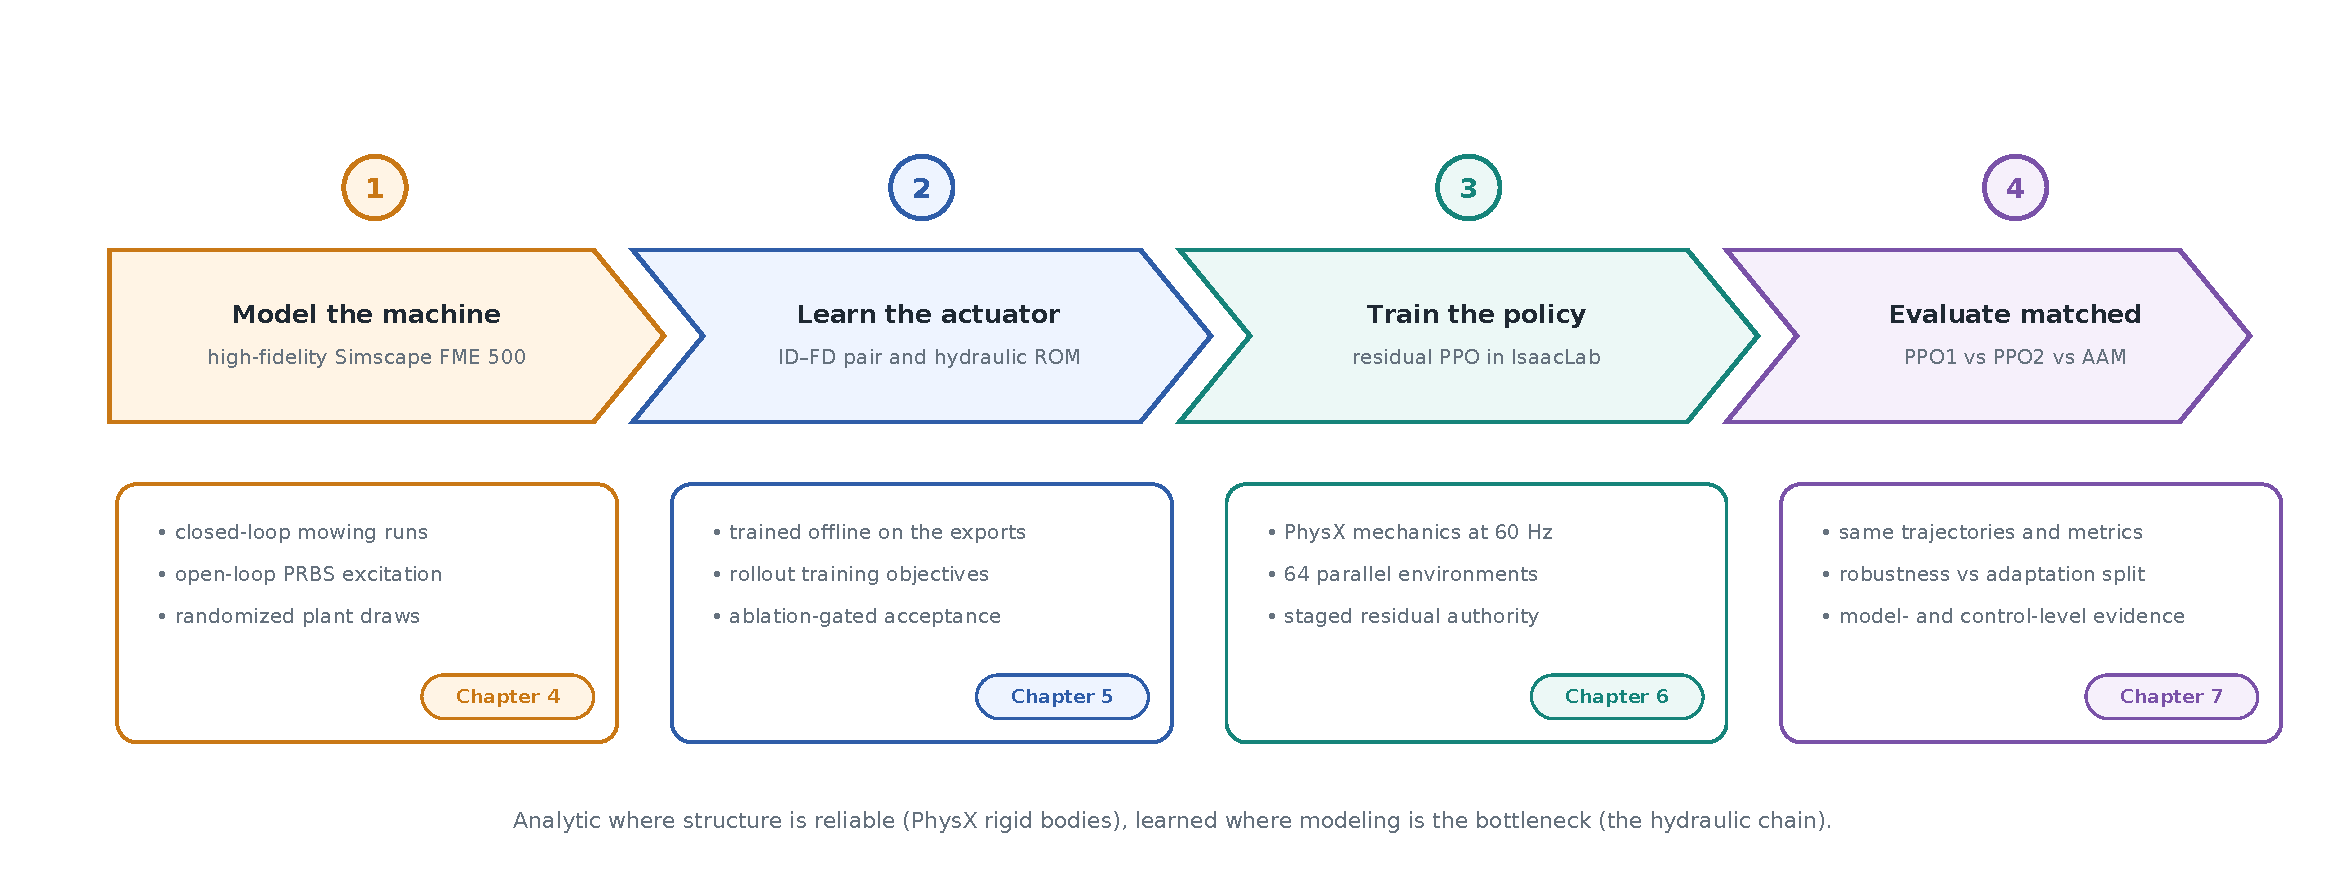
\includegraphics[width=\textwidth]{images/fund_workflow}
  \caption{The four-step workflow of this thesis, following the
  division of labor introduced for legged robots by Hwangbo et
  al.~\cite{hwangbo2019learning}. Each card names what the step contributes and
  the chapter that develops it.}
  \label{fig:fund:workflow}
\end{figure}

\section{Domain Randomization and Latent Adaptation}
\label{sec:fund:domain-randomization}

\subsection{Robustness Through Randomized Training}

A model or policy trained on one simulated plant inherits every
parameter of that plant as an implicit assumption. Domain randomization
attacks this brittleness by training across a distribution of plants,
originally over visual appearance for
perception~\cite{tobin2017domain}, soon after over dynamics parameters
such as masses, frictions, gains, and latencies for
control~\cite{peng2018sim}. The now-standard reading of those results is
that a policy or model that must succeed on many plants converges to
behavior that is \emph{robust} across the family. For the hydraulic arm
the corresponding family is physically meaningful rather than
synthetic: effective bulk modulus varies with entrained air and
temperature, valve gains and leakage drift with wear, and payload
changes with the mounted attachment. Chapter~\ref{chap:data} defines the
randomized parameter space along these same axes.

\subsection{From Robustness to Adaptation}

\begin{figure}[tb]
  \centering
  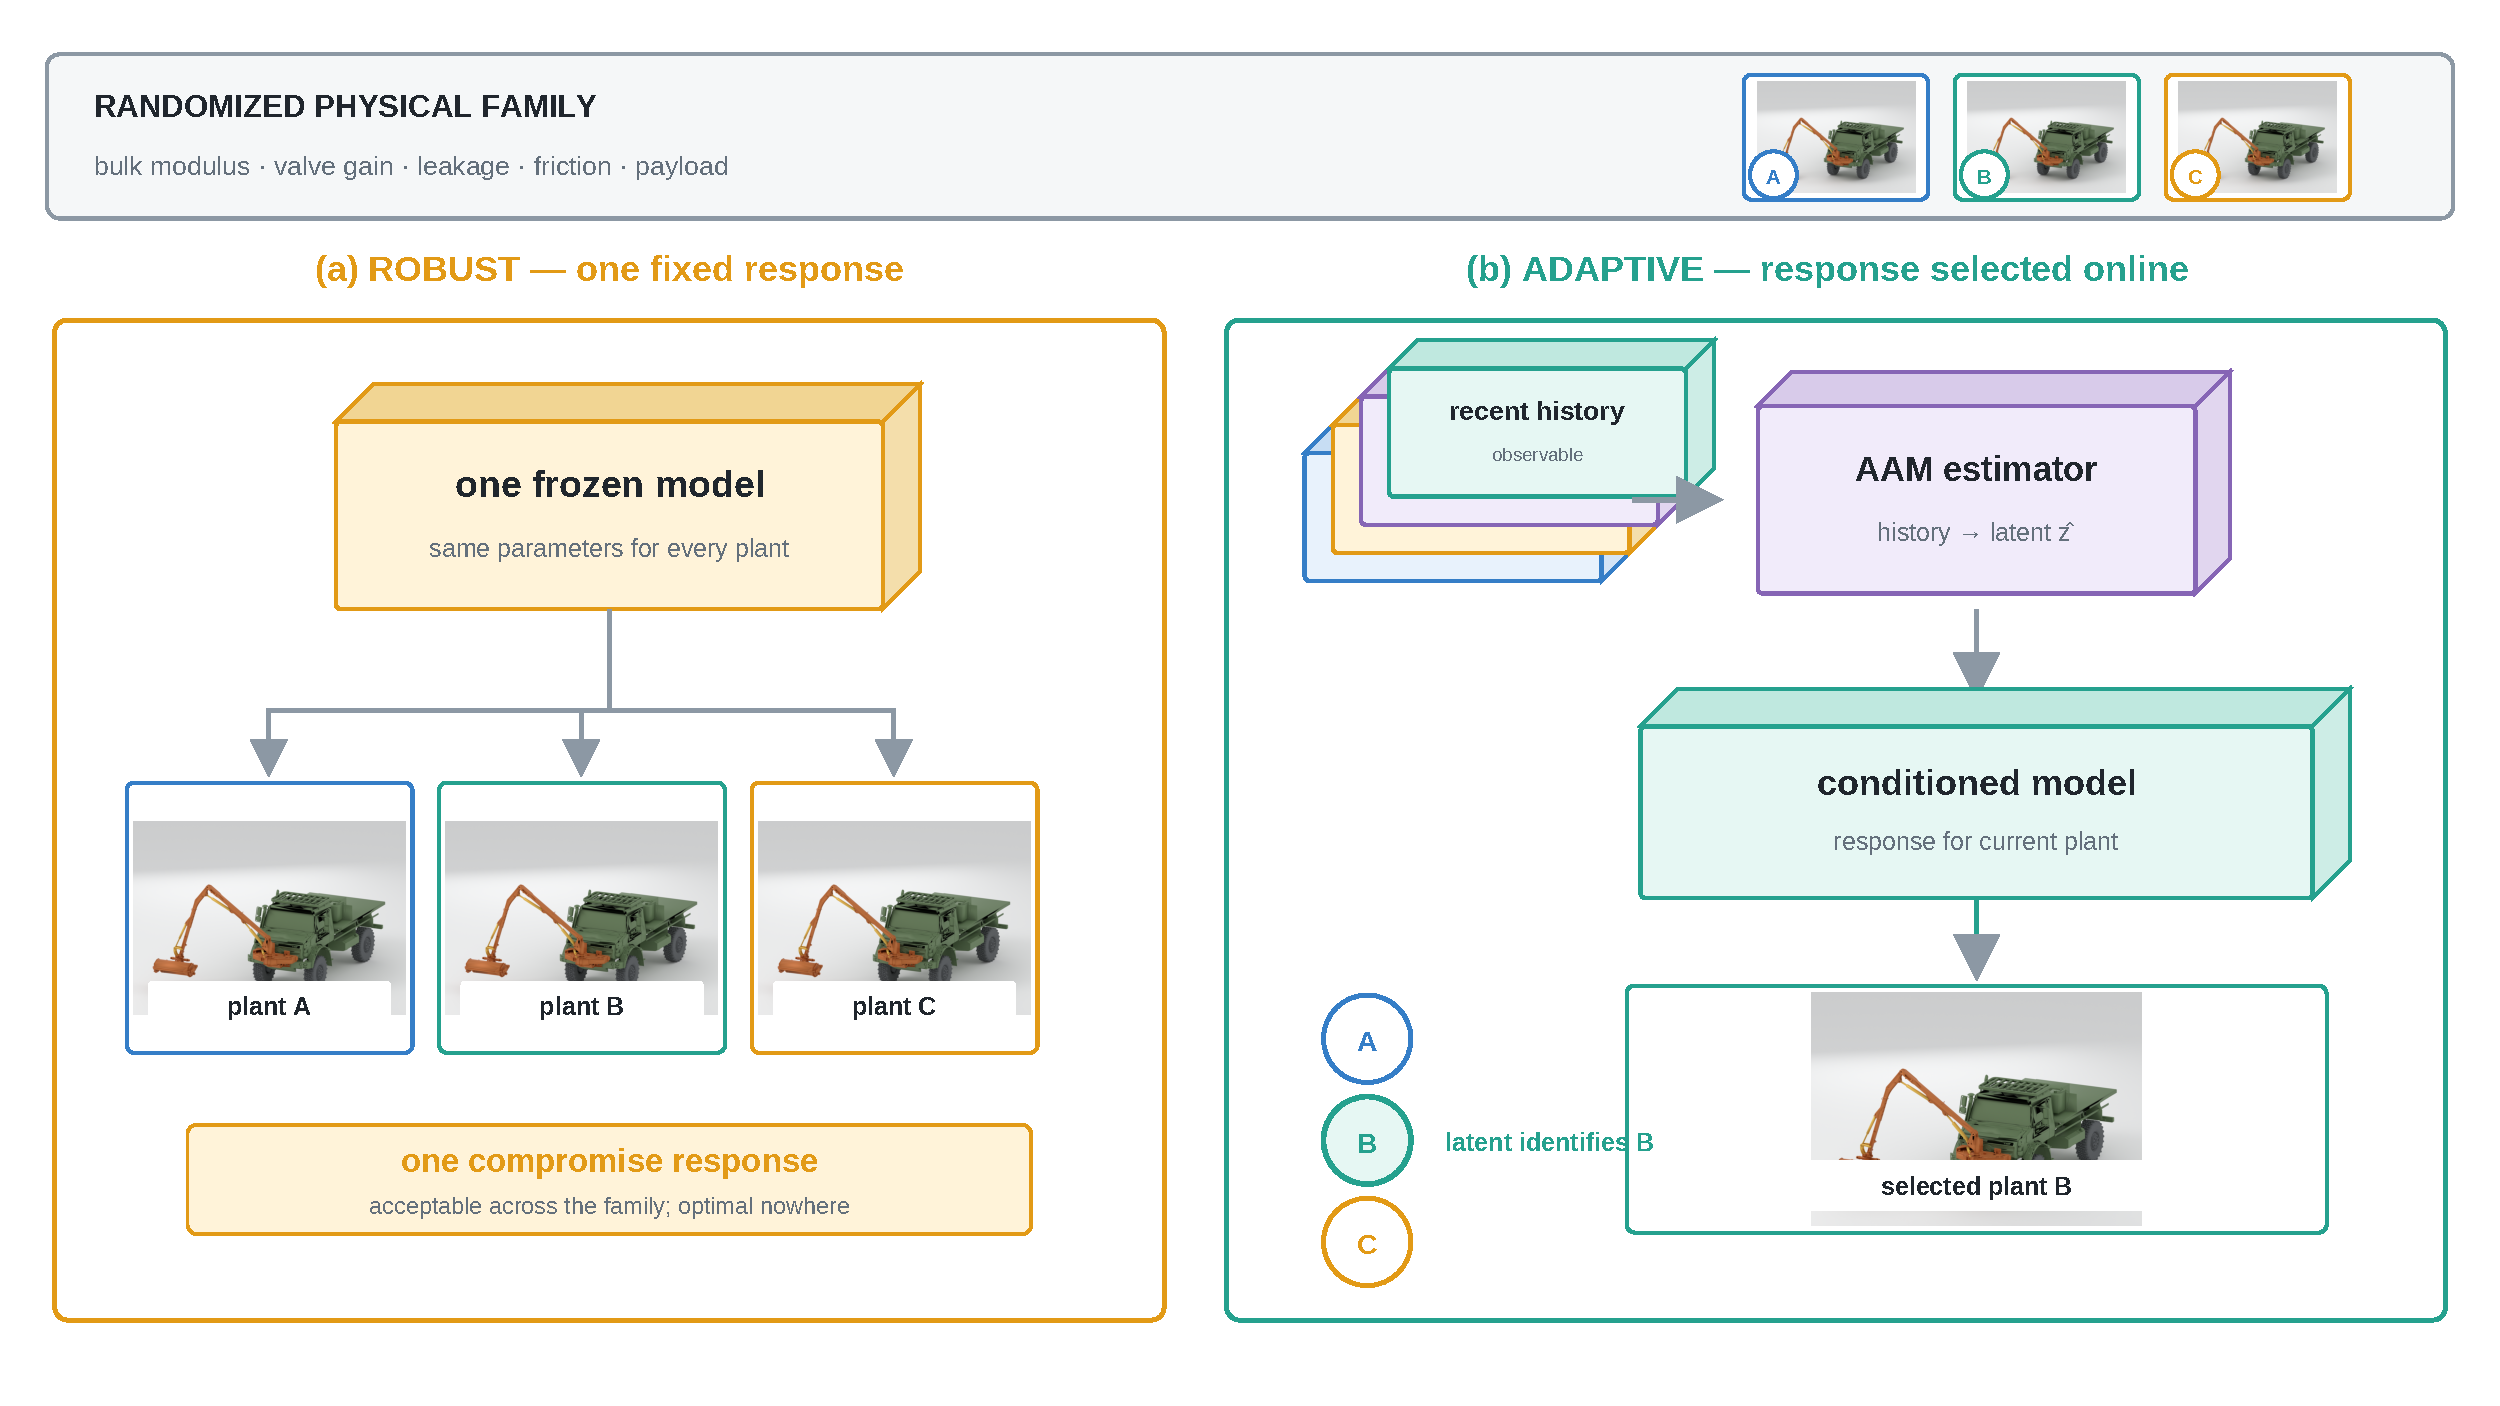
\includegraphics[width=\textwidth]{images/fund_robust_adaptive}
  \caption{Two treatments of the same randomized plant
  family. (a)~Randomized training alone gives a \emph{robust} model: one fixed
  response, acceptable everywhere and optimal nowhere. (b)~Latent conditioning
  adds \emph{adaptation}: an estimator infers $\hat{\bm{z}}$ from recent
  measured history and the model changes its response. The estimator is trained
  against a privileged latent but deploys on observable signals alone.}
  \label{fig:fund:robust-adaptive}
\end{figure}

Robustness, however, is a compromise by definition: one response that is
acceptable everywhere is optimal nowhere. The alternative is to let the
controller or model identify which member of the family it is currently
facing and condition on that estimate
(Figure~\ref{fig:fund:robust-adaptive}). The teacher--student
construction makes this trainable. During simulation the true randomized
factors $\factorvec$ are known, and a privileged encoder compresses
them, or their dynamic consequences, into a low-dimensional latent
$\bm{z}$. A
student module then learns to regress $\bm{z}$ from signals that exist
outside simulation, namely the recent history of states, commands, and
responses. Lee et al.~\cite{lee2020learning} used this scheme to walk
over terrain whose properties the robot cannot observe directly. Kumar et al.~\cite{kumar2021rma} sharpened it into rapid motor adaptation.
A first phase trains the policy together with an encoder of the privileged
environment parameters. A second phase trains an adaptation module to recover
the same latent from the observable state--action history. At deployment only
the history-based estimate is used, so the system adapts within fractions of a
second and takes no gradient steps. Classical adaptive control pursues the same goal through online
parameter estimation~\cite{astrom1995adaptive}. The learned variant
replaces explicit parameter estimates with a task-shaped latent, trading
physical interpretability for the ability to summarize many interacting
parameters at once. The construction has since been carried into the
dynamics model itself rather than the policy. Yu et
al.~\cite{yu2026context} condition a neural-ODE dynamics model on a
context vector inferred from state--action history, so the learned model
rather than the controller is what adapts to the current plant. That is
the position the AAM occupies here, and the reason this thesis measures
the adaptation effect at the actuator layer instead of inside the
policy.

The Arm Adaptation Module (AAM) of this thesis
(Chapter~\ref{chap:models}) is this construction applied to hydraulic
actuation, following the adaptive path of
Figure~\ref{fig:fund:robust-adaptive}(b). The privileged latent
$\bm{z} = \mu(\factorvec)$ is a two-dimensional compression of the
physical factor vector $\factorvec$, validated by the system-dynamics
surrogate of Chapter~\ref{chap:models}. The AAM reads its deployable
estimate $\latenthat$ from a quarter second of causal, observable
cylinder-signal history.

Where that estimate is \emph{used} is a design decision that this thesis
fixes explicitly, because it is easy to state loosely. The latent does
not condition the reduced-order model. In the proposed stack,
\ppoIDAAMFD, the inferred latent conditions a small bounded residual
adapter around the \emph{frozen inverse-dynamics model}, leaving the
forward model, the policy, and the PhysX plant unchanged. Conditioning
the policy directly on $\latenthat$ is treated as an ablation rather
than the default design (Chapter~\ref{chap:evaluation}). Two claims are
therefore kept apart throughout. A model trained across randomized
plants is \emph{robust}, not automatically adaptive, and evidence that a
\emph{privileged} latent carries useful dynamics information is not
evidence that an \emph{inferred} one improves control. Collapsing either
pair is a common confound in the sim-to-real literature, and the
experimental design of Chapter~\ref{chap:evaluation} is built to avoid
both.

\section{Reinforcement Learning and Structured Priors}
\label{sec:fund:rl-residual}

\subsection{Policy Optimization}

Reinforcement learning frames control as sequential decision making: a
policy $\pi_\vartheta(\bm{a}\,|\,\bm{o})$ maps observations to actions
and is optimized to maximize expected cumulated
reward~\cite{sutton2018reinforcement}. Among policy-gradient methods,
proximal policy optimization (PPO)~\cite{schulman2017proximal} has
become the default in robot learning for its simplicity and stable
large-batch behavior. It constrains each update through a clipped surrogate objective, which
limits how far the ratio between the new and the old policy may move before
the improvement term stops paying. Advantages are estimated with generalized
advantage estimation~\cite{schulman2016gae}. The objective as configured for
this thesis is written out in Section~\ref{sec:ctrl:optimization}. What makes
on-policy methods like PPO practical for this thesis is throughput.
GPU-parallel simulators run thousands of environment instances at
once~\cite{makoviychuk2021isaac}, and locomotion policies have been
trained this way in minutes~\cite{rudin2022learning}. This is the regime
in which the full hydraulic model cannot run
(Section~\ref{sec:fund:sim-data-source}) and the learned actuator
surrogates can.

\subsection{Structured Priors for Policy Learning}
\label{sec:fund:prior}

Applying RL to the mowing arm from scratch would discard the reliable
kinematic structure of Section~\ref{sec:fund:kinematics} and force the policy
to rediscover it from reward, with excursions a heavy boom cannot afford.
Three constructions inject that structure, and they differ in \emph{when} the
classical controller acts.

Residual reinforcement learning adds the policy output to a hand-designed
controller's command at
runtime~\cite{johannink2019residual,silver2018residual}, with the policy
restricted to a bounded band. The nominal controller provides competent
behavior from the first step, but it remains in the deployed loop, so every
result is a property of the pair. Policy distillation moves the prior to
training time instead: a privileged teacher, here the DLS controller reading
quantities the deployed system cannot, generates demonstrations, and the
student is fitted to them by supervised imitation before any reward is
optimized~\cite{ross2011reduction}. At deployment the teacher is gone and the
student is the whole controller. The third construction, developed in
Section~\ref{sec:ctrl:anchored}, keeps the prior for the whole of
optimization without returning it to the runtime loop. The distilled student
is frozen as a \emph{reference} policy and reward optimization is restricted
to a neighbourhood of it, measured as a divergence between the two action
distributions and evaluated only on states the learner itself visits.

This thesis uses the second and third. The deployed policy of all three
stacks is a \emph{sole} cylinder-motion controller, emitting the desired
cylinder command with no nominal command added at runtime, and the DLS
controller is retained only as teacher and as the closed-loop controller
during identification. What bounds exploration is therefore not a residual
band but the action contract itself, specified in
Chapter~\ref{chap:control}.

Improving a policy that a simulator has already made competent is an active
question. Yin et al.~\cite{yin2025rapidly} retain the value function learned
in simulation to guide exploration during real-world fine-tuning, treating
the simulator as a source of structure rather than a plant to be abandoned.
This thesis shares that premise and differs in what is retained: the policy
itself, held as a fixed reference that bounds how far reward optimization may
travel.

That construction answers a measured result rather than a design assumption.
\emph{Unconstrained} PPO fine-tuning from the distilled student raised total
reward while degrading the primary tracking objective, consistently enough
that distillation was for several development cycles treated as the
\emph{endpoint} rather than an initialization. The diagnosis is a mismatch of
objectives rather than a failure of the optimizer: the reward is a proxy,
acceptance is decided by physical gates, and the reward's optimum does not
lie inside the gate-feasible set (Section~\ref{sec:ctrl:training}). Anchoring
is what allows the reported \ppoROM{} policy to be a fine-tuned actor rather
than a distilled one.

\subsection{Reinforcement Learning on Hydraulic Machines}

Applications of deep RL to hydraulically actuated arms are still few,
and the closest of them sharpen rather than close the gap this thesis
addresses. Egli and Hutter demonstrated RL-based trajectory tracking for
the arm of a full-size hydraulic excavator, first in
simulation-to-machine transfer experiments~\cite{egli2020towards} and
then as a general automation approach deployed on a walking
excavator~\cite{egli2022general}. Spinelli et
al.~\cite{spinelli2024rl} extended that line to material handlers whose
tool is underactuated, training in simulation and validating on a
commercial machine, which shows the approach scales to arms where part
of the mechanism is not directly commanded. The mowing head of this
thesis is underactuated in the same sense, through its passive swivel
joint. Maitan et al.~\cite{maitan2026contraction} attacked the problem
from the opposite end, learning force control for a single hydraulic
actuator directly on hardware and constraining exploration with a
contraction-metric filter so that training on a real cylinder stays
safe. Their work is the closest published statement of the difficulty
this thesis handles in simulation: an unconstrained policy acting on a
hydraulic cylinder is not safe by default, and something must bound it.
Their key ingredient is shared with
this work: a data-driven model of the machine's actuator response,
learned from recorded operation and used as the training plant for the
policy. The differences define where this thesis stands. Their actuator
model is identified for one physical machine, so robustness across a
plant family and online adaptation to a changing plant are outside its
scope. Their policy is trained against that single model without a
privileged teacher supplying the structured prior. And their evaluation
compares against human operators and classical baselines rather than
isolating the contribution of the actuator representation itself. The
comparison that Chapter~\ref{chap:evaluation} is built around (same task, same policy architecture, same observation and action contracts,
same terrain, reward, seeds and training budget, with only the actuator and adaptation path differing) has to the author's knowledge no
published counterpart for hydraulic manipulators.

One property of a learned policy over a learned actuator cuts both ways
and shapes the evaluation methodology of this thesis. Because the policy
can compensate for a mediocre actuator model, closed-loop tracking error
alone cannot distinguish a good model from a good patch over a bad one.
The protocol of Chapter~\ref{chap:evaluation} therefore reports
model-level rollout metrics, the magnitude and smoothness of the emitted
commands, and the standing cylinder-tracking and actuator-prediction
residuals alongside task error. A better actuator representation must show up as a smaller standing model error and
quieter commands, not merely as equal tracking.

\section{Research Gap and Thesis Positioning}
\label{sec:fund:gap}

Laid side by side, the threads of this chapter each solve part of the
problem and leave a specific remainder
(Table~\ref{tab:fund:positioning} names the works). Hydraulic control
theory provides structure and explains why fixed models fail, but its
precise methods presuppose plant knowledge that a commercial mowing
implement does not come with. Learned dynamics models replace
derivation with data, but the identifiability literature, and the
measured failure recounted in Section~\ref{sec:fund:identifiability},
shows that closed-loop operation data silently produces models without
control authority. Learned actuator surrogates embedded in parallel
simulation are proven for electric drives but not for actuators
dominated by pressure dynamics, relief saturation, and valve dead
zones. Domain randomization yields robustness, and the teacher--student
construction yields fast online adaptation, but these results live
almost entirely in locomotion, where the adapted quantity is the
contact with the world rather than the actuator itself. RL has reached
full-size hydraulic arms, but without a structured prior, without
adaptation, and without isolating the actuator representation.
Residual RL and policy distillation both integrate learning with a
structured controller, yet published evaluations rarely control for the
fact that the policy can mask actuator-model deficiencies.

\begin{table}[tb]
  \centering
  \caption{Positioning of this thesis against the reviewed lines of work.
  Columns: (I)~learned model of \emph{hydraulic} actuator dynamics;
  (II)~training data audited for causal input identifiability;
  (III)~online latent adaptation to a changing plant; (IV)~structured
  classical controller retained as a prior, with bounded action
  authority; (V)~matched comparison isolating the actuator
  representation.
  ($\checkmark$)~=~partially or implicitly addressed.}
  \label{tab:fund:positioning}
  \small
  \begin{tabular}{lccccc}
    \toprule
    Line of work & I & II & III & IV & V \\
    \midrule
    Model-based hydraulic control~\cite{mattila2017survey,jelali2003hydraulic}
      & --- & ($\checkmark$) & ($\checkmark$) & $\checkmark$ & --- \\
    Actuator networks for legged robots~\cite{hwangbo2019learning,rudin2022learning,yamamori2026actuator}
      & --- & $\checkmark$ & --- & --- & --- \\
    RL for hydraulic machines~\cite{egli2020towards,egli2022general,spinelli2024rl,maitan2026contraction}
      & $\checkmark$ & ($\checkmark$) & --- & --- & --- \\
    Latent online adaptation~\cite{lee2020learning,kumar2021rma,yu2026context}
      & --- & --- & $\checkmark$ & --- & --- \\
    Residual RL and policy
    distillation~\cite{johannink2019residual,silver2018residual,ross2011reduction,yin2025rapidly}
      & --- & --- & --- & $\checkmark$ & --- \\
    \midrule
    This thesis (\ppoROM{} / \ppoIDFD{} / \ppoIDAAMFD)
      & $\checkmark$ & $\checkmark$ & $\checkmark$ & $\checkmark$ & $\checkmark$ \\
    \bottomrule
  \end{tabular}
\end{table}

What is missing is the combination, summarized in
Table~\ref{tab:fund:positioning}: cylinder-space actuator dynamics learned
from deliberately identifiable data, reduced to a physics-structured
command-conditioned model fast enough for massively parallel policy
training, carrying a dynamics latent that is validated before deployment
and recovered online from observable history alone, and evaluated in a
framework where adaptive and non-adaptive actuator representations are
compared under matched conditions. Assembling this on the MULAG FME~500
mowing arm is the contribution of this thesis. It takes the form of three
control stacks differing \emph{only} in the actuation and adaptation path
between the policy's cylinder command and PhysX:

\begin{description}
  \item[\ppoROM.] The policy commands desired cylinder motion, which the
    validated command-conditioned reduced-order model realizes. This is
    the certified actuator baseline and the current shippable stack.
  \item[\ppoIDFD.] The same policy interface drives the frozen inverse
    model followed by the validated strict forward model. This is the
    non-adaptive learned baseline. It tracks the line more finely than
    \ppoROM{} and fails the ground-contact requirement, which makes it an informative negative result rather than a weaker copy.
  \item[\ppoIDAAMFD.] The AAM infers a dynamics latent from causal
    observable history, and that latent conditions a small bounded
    residual adapter around the frozen inverse model before the same
    frozen forward model and PhysX. This is the proposed adaptive
    method.
\end{description}

The scientific variable is therefore the actuator and adaptation path
alone, with task, observation and action contracts, terrain, reward,
training budget, test factors, seeds and acceptance gates held matched.
Robustness and adaptation are measured as separate effects rather than
conflated ones. The next chapter grounds this program in the concrete
system.
